\documentclass[../STS.tex]{subfiles}



\begin{document}

\section{Boxplot}

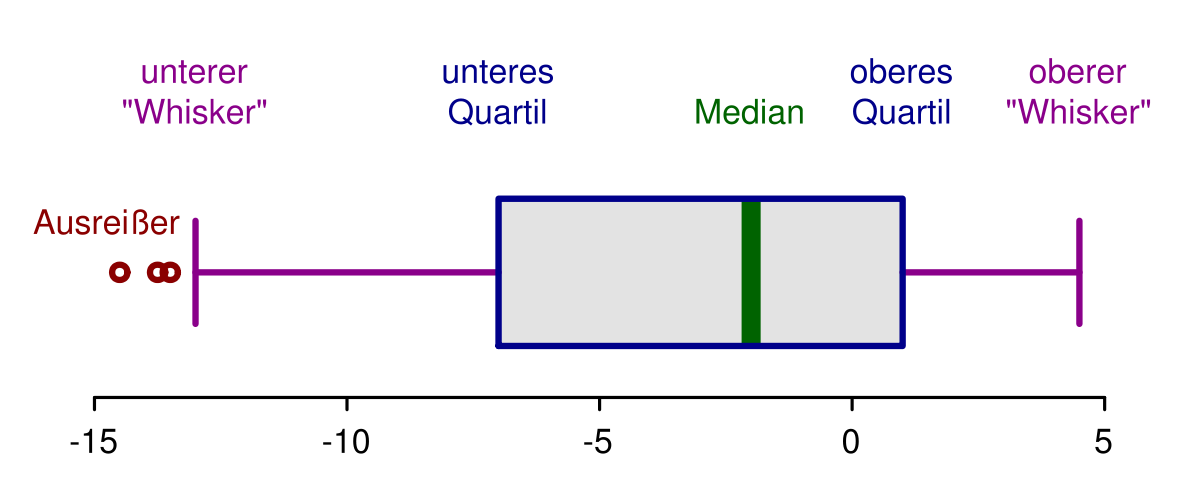
\includegraphics[height=6cm]{IMG_0206}
	

\begin{tabular}{|c c c|}

\hline
Beschreibung & Formelzeichen & Berechnung \\

\hline

	Unterer Whisker &
	&
	maximal, sonst Daten
	$
	Q_1 - 1.5 * I_{QR}
	$ \\
	\hline
	
	Obrerer Whisker &
	&
	maximal, sonst Daten
	$
	Q_3 + 1.5 * I_{QR}
	$
	\\
	\hline
	
	0.25er Quantil &
	$ Q_1 $ &
	\\
	\hline
	
	0.75er Quantil &
	$ Q_3 $ &
	\\
	\hline
	
	Interquartilsabstand &
	$ I_{QR} $ &
	\\
	\hline
	
	Median &
	$ X_{med} $ &
	\\
	\hline
	
	Modulo Wert &
	$ X_{mod} $ &
	Höchster Stichprobenwert (Spitze der Kurve)
	\\
	\hline
	
\end{tabular}
	

	\subsection{Quantil}

	
	\subsubsection{Wenn $n \cdot q $ eine ganze Zahl ist}
	$
	R_q
	=
	\frac{1}{2}
	\cdot
	(
		X_{n \cdot q} +
		X_{n \cdot q+1}
	)
	$

\subsubsection{Wenn $n \cdot q $ keine Ganze Zahl ist}
	$
	X_{| n \cdot q |}
	$
	mit $ n \cdot q $ die n\"achstgrösste Zahl
	
\subsection{Boxplot in einer Klasse}
1. CDF in der Verteilung berechnen \\
2. Klasse auswählen für die $ F(a) \leq q < F(b) $


$
\frac{F(b) - F(a)}{b-a} = \frac{q - F(a)}{R_q - a}
$
\\
Nach $ R_q $ umgestellt

$
R_q = a + \frac{b-a}{F(b)-F(a)}[q - F(a)]
$

\subsection{Median}
Der in der Mitte liegende Wert einer sortierten Datenmenge

\subsubsection{Wenn $ n $ gerade}

$
X_{med} = x[\frac{n+1}{2}]
$

\subsubsection{Wenn $ n $ ungerade}

$
X_{med} =
\frac{1}{2} [X_{[\frac{n}{2}]} + X_{[\frac{n}{2} + 1]}]
$

	
\end{document}



